\documentclass{beamer}
\usepackage[utf8]{inputenc}
\usepackage[]{amsmath}
\usepackage{graphicx}
\usepackage{subcaption} % package pour faire des subfigures
\usepackage{multirow} % package pour multirow/multicolumn
\usepackage{booktabs} % package pour top/mid/bottom rule
\usepackage{tcolorbox} % toujours plus de boites
\usepackage[backend=biber]{biblatex}


\addbibresource{Biblio_dbl_quantum.bib}

%\bibliographystyle{stylename}
%\bibliography{Biblio_dbl_quantum}

\title{Group meeting : Cross-relaxation with NV centers ensemble in diamond}
%\author{Clément Pellet-Mary\\ Laboratoire de physique de l'ENS\\ \textit{ENS, Paris}}
\date\today

\mode<presentation> {\usetheme{Rochester}}

\begin{document}
\begin{frame}
\maketitle
\end{frame}
\begin{frame}{The Nitrogen Vacancy Center}
\begin{center}
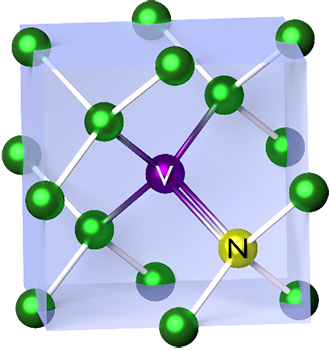
\includegraphics[scale=.4]{Nitrogen-vacancy_center}
\end{center}

\section{The NV center}
\begin{itemize}
\item 0D fluorescent object with ZPL at 638 nm
\item Controllable and readable spin at room temperature (!)
\item Working with 10$^9$ emitters (typ.)
\end{itemize}
\end{frame}
\begin{frame}{NV center : Optical properties}
\centering
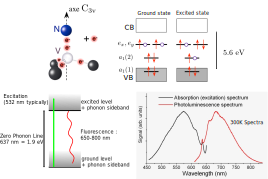
\includegraphics[scale=.4]{slide_NV_optical}
\end{frame}
\begin{frame}{NV center : 8 levels}
\centering
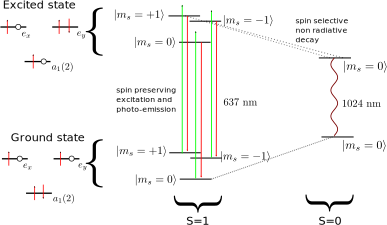
\includegraphics[scale=.3]{NV_8_niveaux}
\end{frame}
\begin{frame}{NV center : 3 levels}
\centering
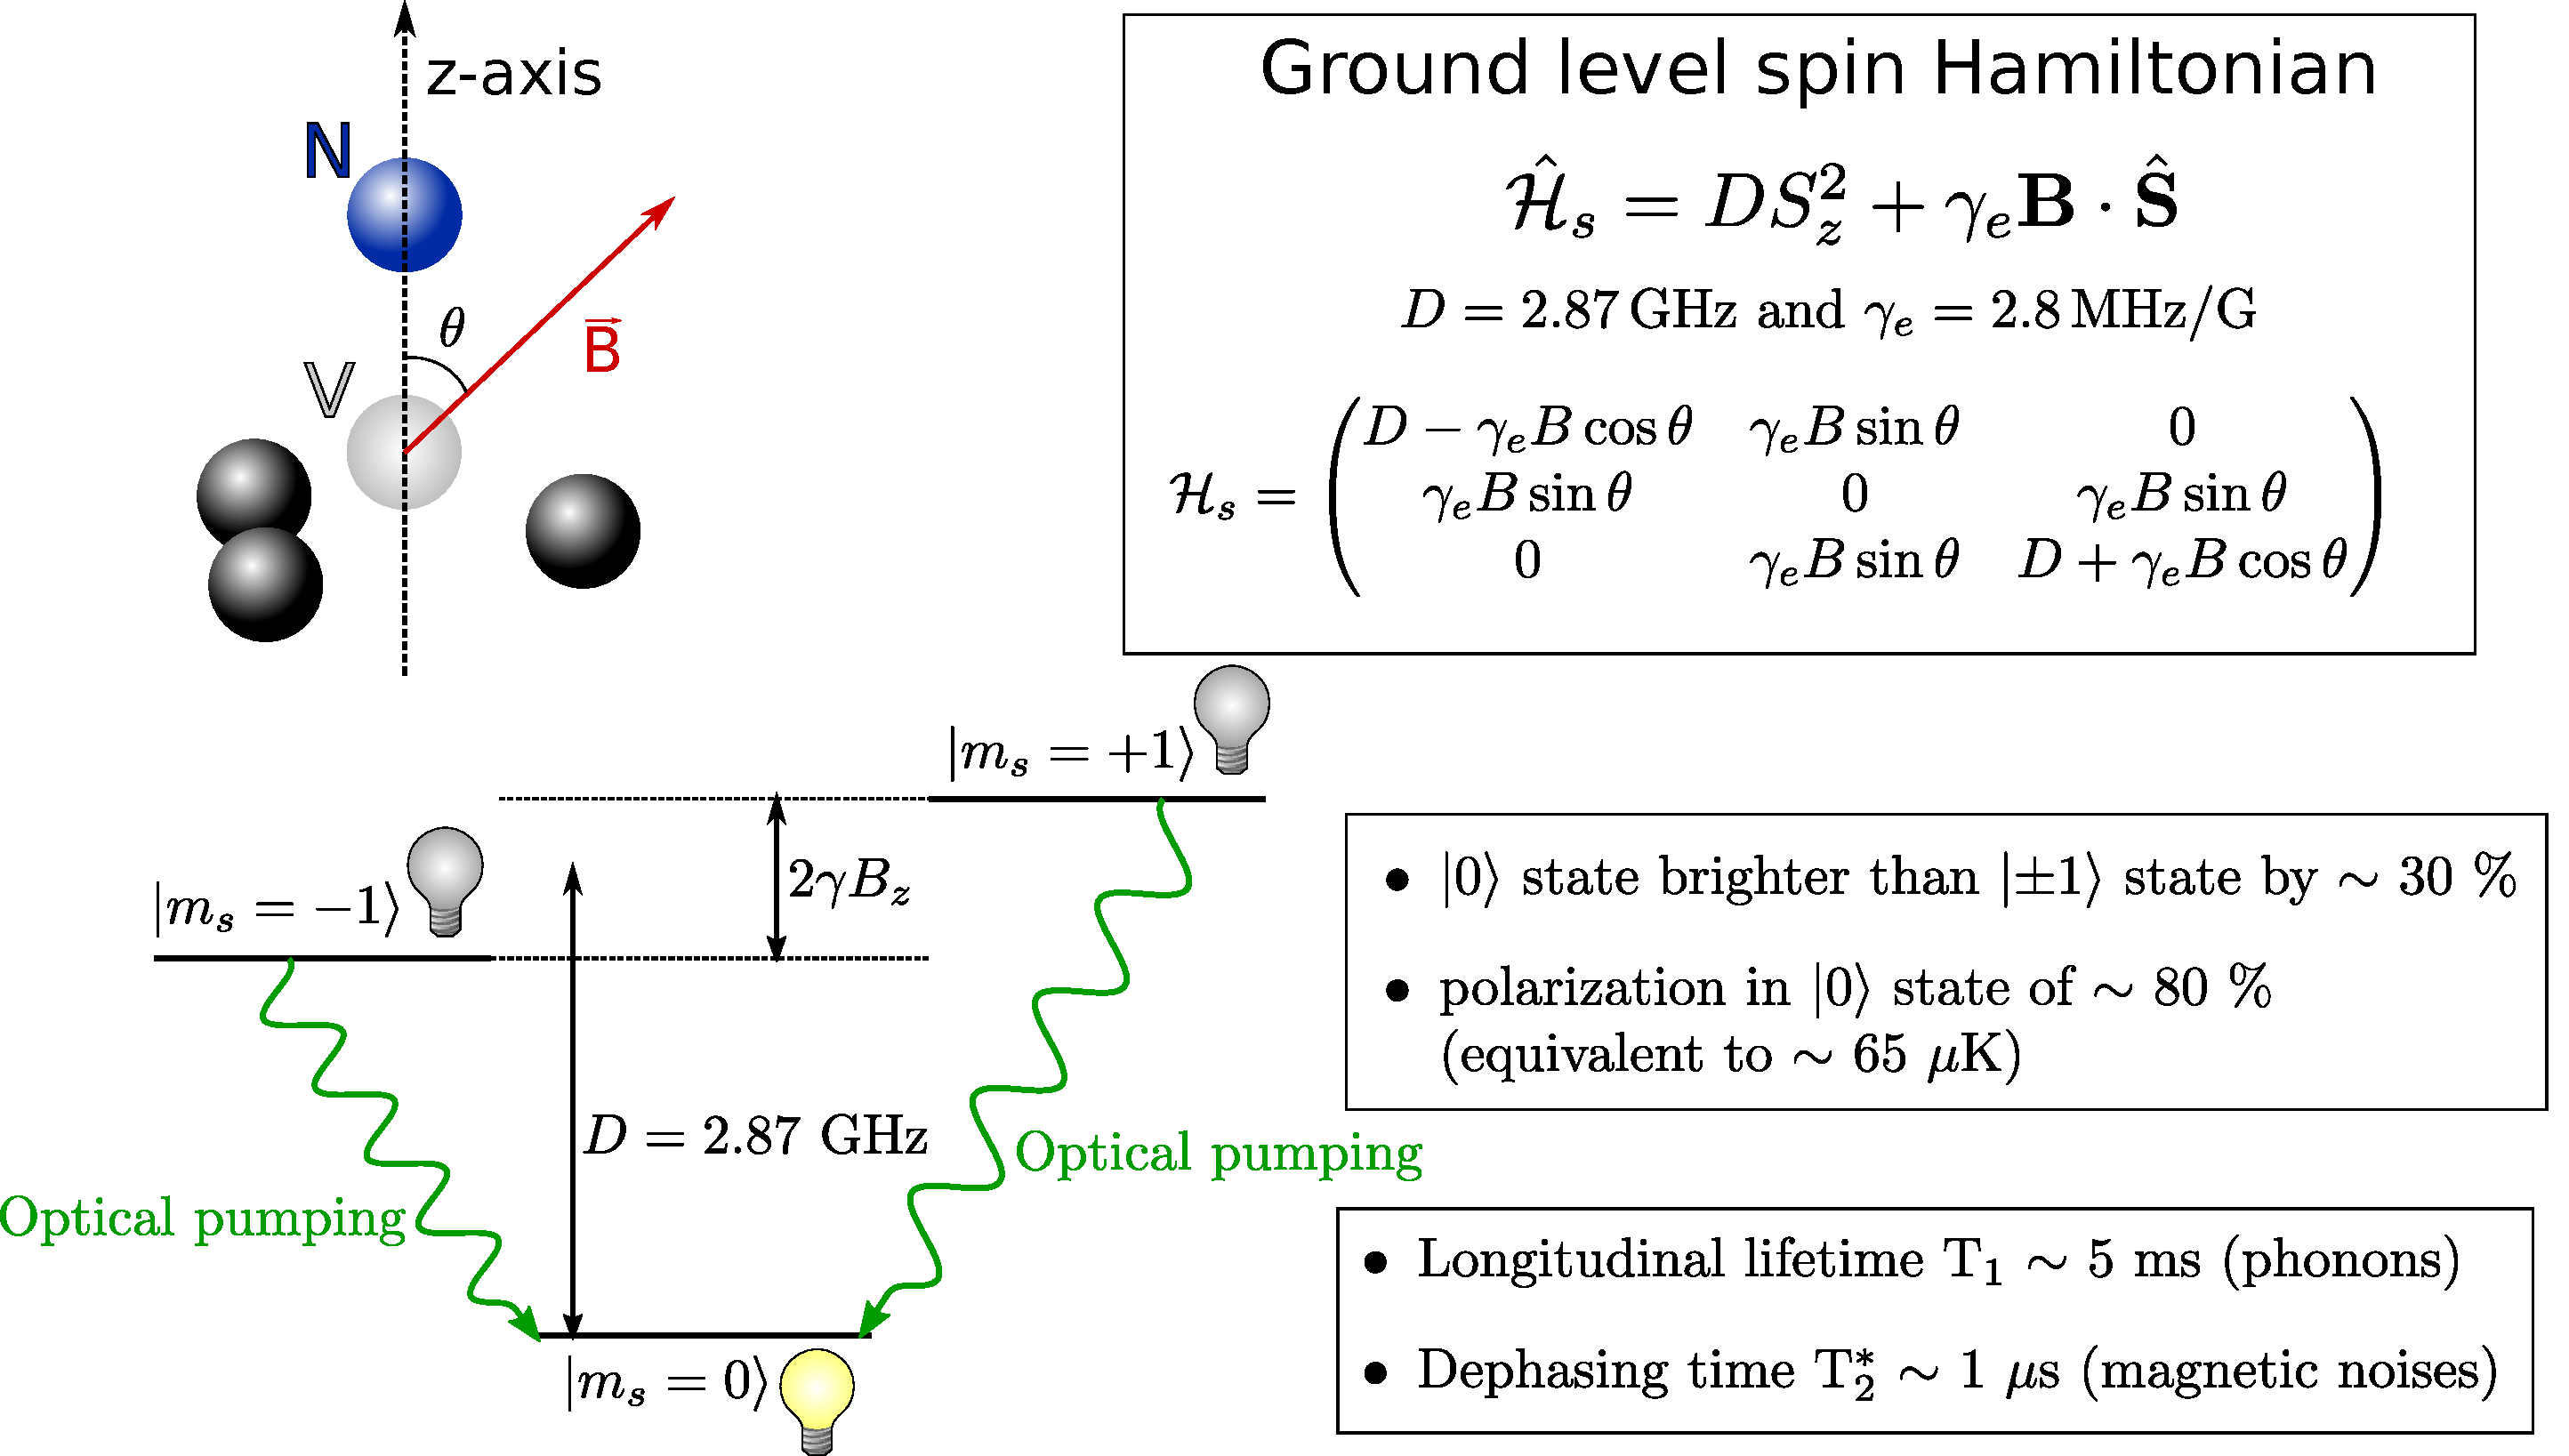
\includegraphics[scale=.23]{slide_3_niveaux}
\end{frame}
\begin{frame}{Spin manipulation}
\centering
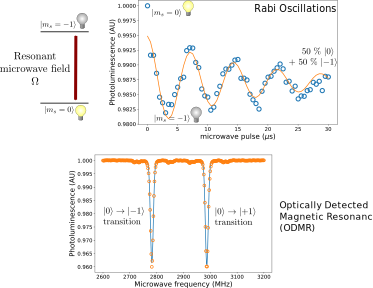
\includegraphics[scale=.25]{slide_rabi_odmr}
\end{frame}
\begin{frame}{Summary : Magnetometry with NV centers}
\centering
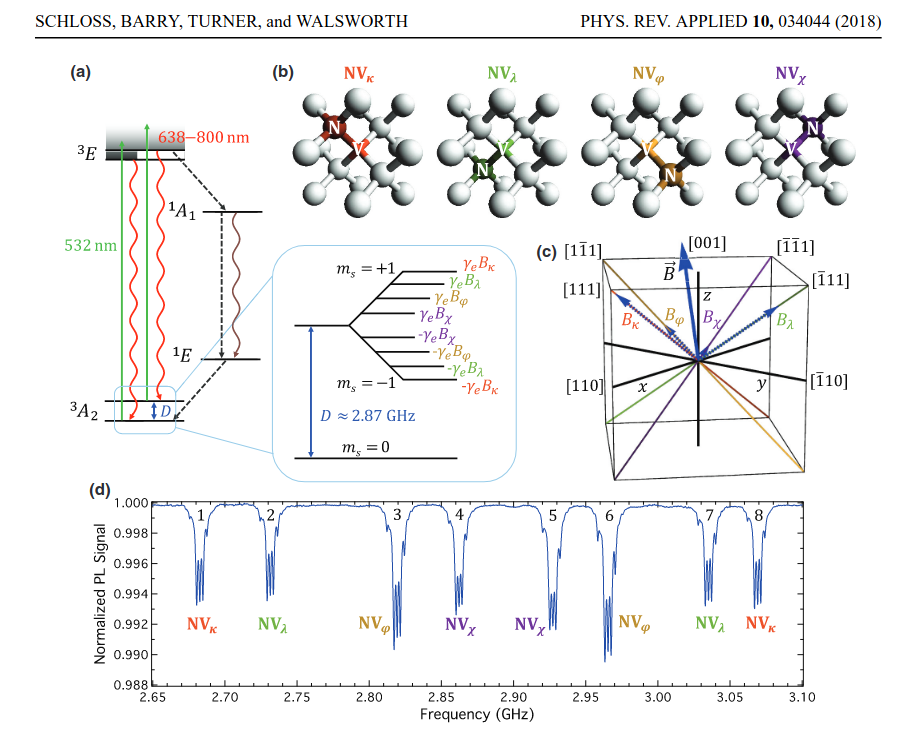
\includegraphics[scale=.4]{ESR_8raies_article}
\end{frame}
\section{Probing dark spins with cross-relaxations}
\begin{frame}{Principle of spin cross-relaxation (CR)}
\centering
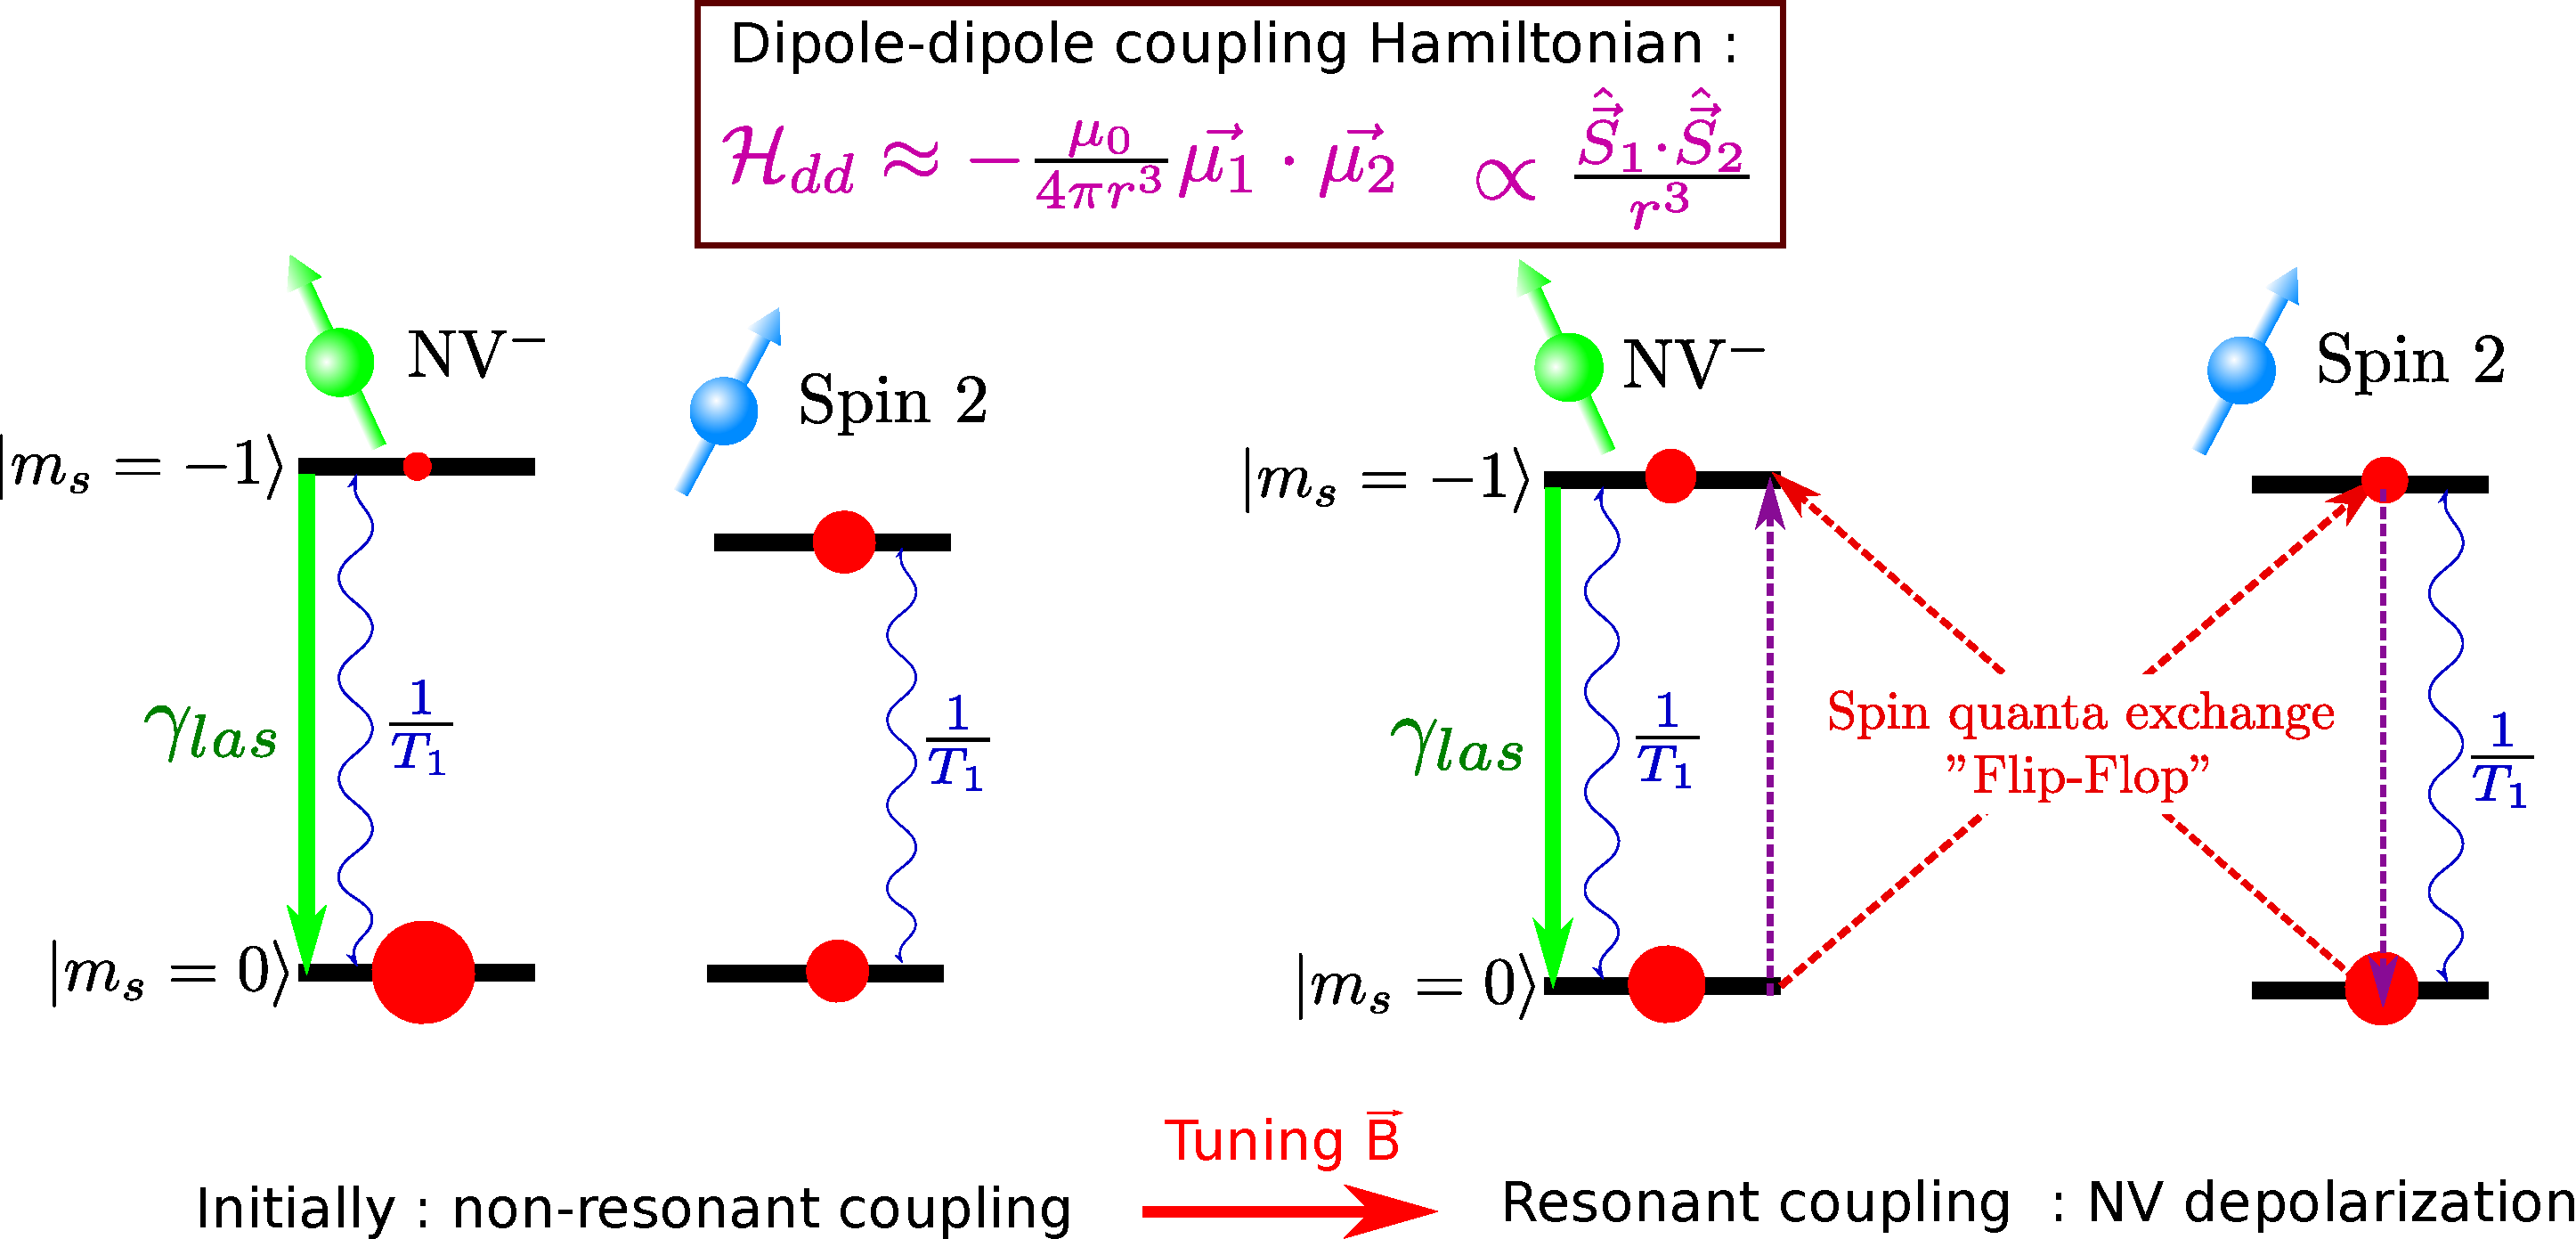
\includegraphics[scale=.23]{Slide_CR}
\end{frame}
\begin{frame}{Detection of dark spins in CVD sample}
\centering
\includegraphics[scale=.35]{Slide_CR_CVD}
\end{frame}
\begin{frame}{NV-NV Cross-Relaxation}
%Le plot avec les 3 trois bosses du CR-méca (+ Mrozek ?)
\end{frame}
\begin{frame}{Mechanically detetcted Cross-Relaxation}
%Le papier CR-méca
\end{frame}
\section{magnetometry with cross-relaxations}
\end{document}